\begin{figure}[t]
\centering
\resizebox{\linewidth}{!}{%
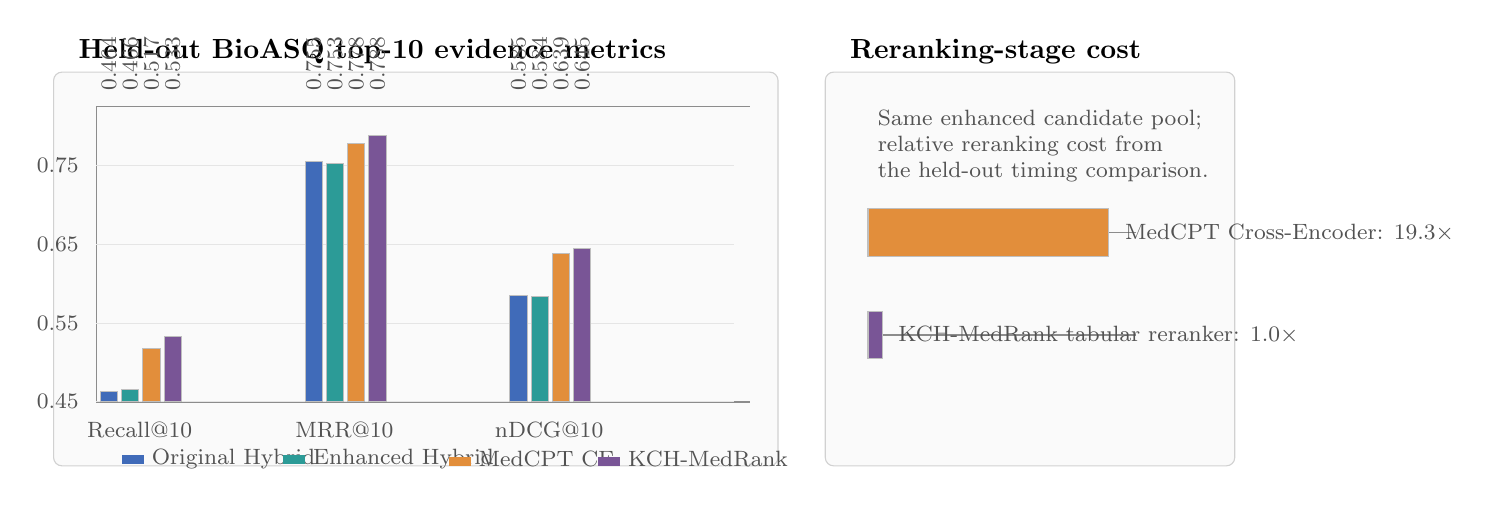
\begin{tikzpicture}[
  font=\small,
  axis/.style={draw=black!45, line width=0.55pt},
  grid/.style={draw=black!10, line width=0.4pt},
  lab/.style={font=\footnotesize, text=black!68},
  panel/.style={draw=black!18, rounded corners=3pt, fill=black!2}
]
\definecolor{kchA}{RGB}{64,107,185}
\definecolor{kchB}{RGB}{44,155,151}
\definecolor{kchC}{RGB}{226,142,59}
\definecolor{kchD}{RGB}{121,85,150}

\begin{scope}
  \node[panel, minimum width=9.2cm, minimum height=5.0cm, anchor=south west] at (-0.55,-0.82) {};
  \node[anchor=west, font=\bfseries] at (-0.35,4.45) {Held-out BioASQ top-10 evidence metrics};
  \draw[axis] (0,0) -- (0,3.75) -- (8.3,3.75);
  \draw[axis] (0,0) -- (8.3,0);
  \foreach \v/\y in {0.45/0,0.55/1,0.65/2,0.75/3} {
    \draw[grid] (0,\y) -- (8.1,\y);
    \node[lab, anchor=east] at (-0.1,\y) {\v};
  }
  \foreach \gx/\name in {0.55/Recall@10,3.15/MRR@10,5.75/nDCG@10} {
    \node[lab] at (\gx,-0.36) {\name};
  }
  \foreach \x/\v/\c in {0.05/0.4636/kchA,0.32/0.4660/kchB,0.59/0.5172/kchC,0.86/0.5332/kchD,
                        2.65/0.7550/kchA,2.92/0.7530/kchB,3.19/0.7775/kchC,3.46/0.7882/kchD,
                        5.25/0.5848/kchA,5.52/0.5844/kchB,5.79/0.6390/kchC,6.06/0.6446/kchD} {
    \pgfmathsetmacro{\h}{(\v-0.45)*10}
    \draw[fill=\c, draw=black!25, line width=0.35pt] (\x,0) rectangle ++(0.22,\h);
  }
  \foreach \x/\txt in {0.16/0.464,0.43/0.466,0.70/0.517,0.97/0.533,
                       2.76/0.755,3.03/0.753,3.30/0.778,3.57/0.788,
                       5.36/0.585,5.63/0.584,5.90/0.639,6.17/0.645} {
    \node[lab, rotate=90, anchor=west] at (\x,3.83) {\txt};
  }
  \node[lab, anchor=west] at (0.2,-0.72) {\textcolor{kchA}{\rule{0.28cm}{0.12cm}} Original Hybrid};
  \node[lab, anchor=west] at (2.25,-0.72) {\textcolor{kchB}{\rule{0.28cm}{0.12cm}} Enhanced Hybrid};
  \node[lab, anchor=west] at (4.35,-0.72) {\textcolor{kchC}{\rule{0.28cm}{0.12cm}} MedCPT CE};
  \node[lab, anchor=west] at (6.25,-0.72) {\textcolor{kchD}{\rule{0.28cm}{0.12cm}} KCH-MedRank};
\end{scope}

\begin{scope}[shift={(9.8,0)}]
  \node[panel, minimum width=5.2cm, minimum height=5.0cm, anchor=south west] at (-0.55,-0.82) {};
  \node[anchor=west, font=\bfseries] at (-0.35,4.45) {Reranking-stage cost};
  \draw[axis] (0,0.85) -- (3.4,0.85);
  \draw[axis] (0,2.15) -- (3.4,2.15);
  \draw[fill=kchD, draw=black!25] (0,0.55) rectangle (0.18,1.15);
  \draw[fill=kchC, draw=black!25] (0,1.85) rectangle (3.05,2.45);
  \node[lab, anchor=west] at (0.26,0.85) {KCH-MedRank tabular reranker: 1.0$\times$};
  \node[lab, anchor=west] at (3.14,2.15) {MedCPT Cross-Encoder: 19.3$\times$};
  \node[lab, align=left, anchor=west] at (0,3.25) {Same enhanced candidate pool;\\relative reranking cost from\\the held-out timing comparison.};
\end{scope}
\end{tikzpicture}}
\caption{Main quantitative picture for the paper. KCH-MedRank improves held-out BioASQ top-10 evidence metrics over Hybrid RRF and MedCPT Cross-Encoder ordering, while the tabular reranking stage is much cheaper than full cross-encoder rescoring on the same candidate pool.}
\label{fig:results-efficiency}
\end{figure}
